\section{Inferring 3D velocities (marginalizing over missing RV
measurements)}
\label{sec:velocities}

It has been demonstrated that the dispersion in vertical velocity, \vz\, for a
group of stars increases with the age of that group (citations).
However, velocities in Galactocentric coordinates, \vx, \vy\ and \vz, can only
be calculated with full 6-D position and velocity information, \ie\ proper
motions, position and radial velocity.
In Angus \etal\ (2020) we showed that kinematic ages can be used to explore
rotational evolution and showed, in the appendix of that paper, that velocity,
\vb\ in the Galactic frame, which can be calculated without an RV measurement,
can be used as an approximation to \vz\ for \kepler\ stars.
This is because the \kepler\ field of view lies at relatively low Galactic
latitudes, ($\sim 5-20$\degrees), so the $z$-direction is similar to the
$b$-direction for \kepler\ stars.
However, \vb\ is only a close approximation to \vz\ at extremely {\it low}
latitudes, and even in the \kepler\ field, kinematic ages calculated with \vb\
instead of \vz\ are systematically larger because of extra noise introduced by
the imperfect translation between \vb\ and \vz .
In this work, we {\it infer} \vz\ by marginalizing over missing RV
measurements.

% Three-dimensional velocities in galactocentric coordinates: \vx, \vy, and \vz\
% can only be directly computed via a transformation from 3D velocities in
% another coordinate system, like the equatorial coordinates provided by \gaia:
% \mura, \mudec, and RV.
% For stars with no measured RV in \gaia\ DR2, \vx, vy, and \vz\ can still be
% inferred from positions and proper motions alone, by marginalizing over
% missing RV measurements.
For each star in our sample, we inferred \vx, \vy, and \vz\ from the 3D
positions and 2D proper motions provided in the \gaia\ DR2 catalog
\citep{brown2011}.
We also simultaneously inferred distance, (instead of using inverse-parallax),
to model velocities \citep[see \eg][]{bailer-jones2015, bailer-jones2018}.

Using Bayes rule, the posterior probability of the parameters given the data
can be written:
\begin{equation}
p(v_{\bf xyz}, D | \mu_{\alpha}, \mu_{\delta}, \alpha, \delta, \pi) =
    p(\mu_{\alpha}, \mu_{\delta}, \alpha, \delta, \pi | v_{\bf xyz}, D)
    p(v_{\bf xyz}) p(D),
\end{equation}
where D is distance, $\alpha$ is Right Ascension (RA), $\delta$ is declination
(dec), $\pi$ is parallax, $\mu_\alpha$ is proper motion in RA, and
$\mu_\delta$ is proper motion in dec.

For each star in the \kepler\ field, we explored the posteriors of these four
parameters using the {\it PyMC3} Hamiltonion Monte Carlo (HMC) sampler
\racomment{(citations)}.

\subsection{The prior}
\label{sec:prior}

\begin{itemize}
    \item{{\bf Why is the prior important?}
Arguably, the trickiest part of this inference is in selecting an appropriate
        prior.
Stellar velocities (in certain directions), inferred without RV measurements
        may be sensitive to the prior.
        }
    \item{{\bf How we calculated the prior.}
We used the mean and covariance of the distance and velocity distributions of
\kepler\ targets {\it with} RV measurements to determine the 4D multivariate
Gaussian prior over $\log$(distance) and velocities.
3D velocities were calculated for every star with an RV measurement from
either \gaia\ or \lamost.
These velocities were then sigma-clipped at the 3-sigma level in all three
dimensions to remove large velocity outliers which may be caused by proper
motion or RV measurements with large errors.
We then calculated the mean and covariance of the multivariate Gaussian
distribution of \vx, \vy, \vz, and $\ln$(Distance).
We used this mean and covariance to construct our multivariate Gaussian prior.
        }
    \item{{\bf Is is important to select the prior carefully.}
Our goal was to infer the velocities of stars without RV measurements using a
prior calculated from stars {\it with} RV measurements.
However, stars with and without RVs are likely to be slightly different
populations, the parameters of which depend on the \gaia\ and \lamost\
selection function.
\racomment{Discuss selection functions.}
In particular, stars without RV measurements are more likely to be faint, and
therefore, less massive.
Lower-mass stars are, on average, older, and have larger velocity dispersions.
So a prior based on the velocity distributions of stars with RVs will not
necessarily reflect the velocities of those without.
        }
    \item{{\bf Testing the prior.}
For this reason, we tested how the choice of prior affected the velocities we
inferred.
We tested two priors: one calculated from the velocity distributions of the
brightest half of the RV sample (\gaia\ $G$-band apparent magnitude $<$ 13.9),
and one from the faintest half ($G > $ 13.9).
We selected the 500 faintest stars from the \gaia-\lamost\ RV sample to test
these two priors on.
We chose the faintest stars as these are the most likely to be similar to the
non-RV sample, and to enlarge the difference between the bright prior and the
test sample.
The results of this test are shown in figure \ref{fig:prior_test}
        }
    \item{{\bf Although the prior isn't perfect, it's good
        enough for our study.}}
\end{itemize}


\begin{figure}[ht!]
\caption{
    }
  \centering
    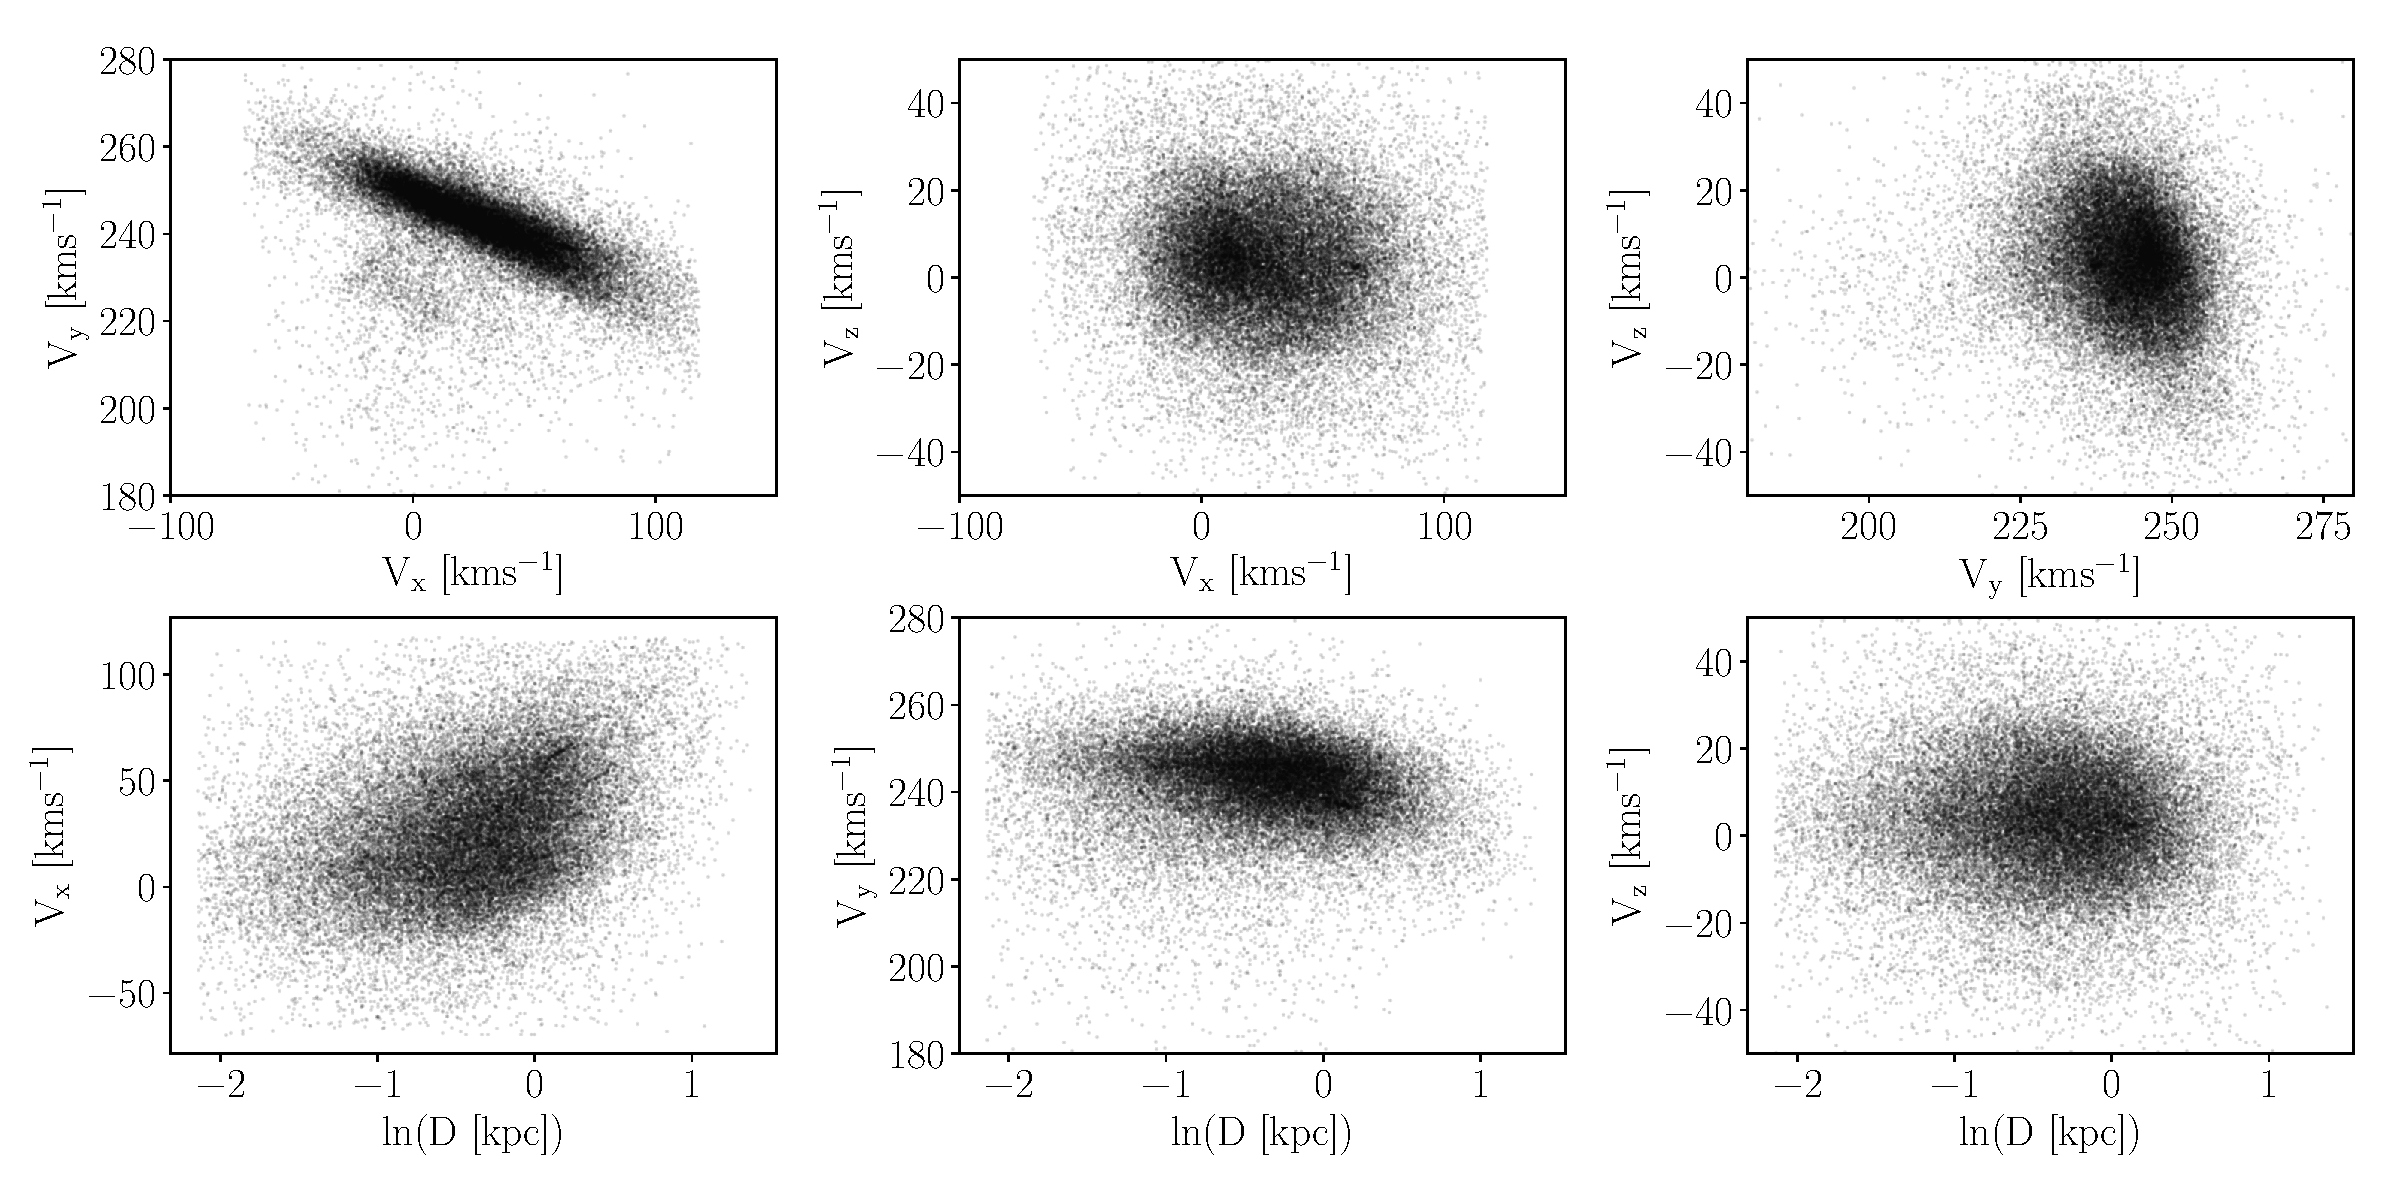
\includegraphics[width=1\textwidth]{prior_distributions}
\label{fig:prior_distributions}
\end{figure}

We tuned the {\it PyMC3} model for 1500 steps, with a target acceptance
fraction of 0.9.
The model was then run for 1000 steps with 4 chains.

Figure \ref{fig:residuals} shows the \vx, \vy\ and \vz\ velocities we
inferred, compared with those calculated from measured RVs.
2000 stars are shown, which were chosen at random from the \kepler\ rotators
with RV measurements.
\begin{figure}[ht!]
\caption{Vertical velocities calculated with full 6D information vs vertical
    velocities inferred without RV, for all 3000 \mct\ stars with \gaia\ RV
    measurements.}
  \centering
    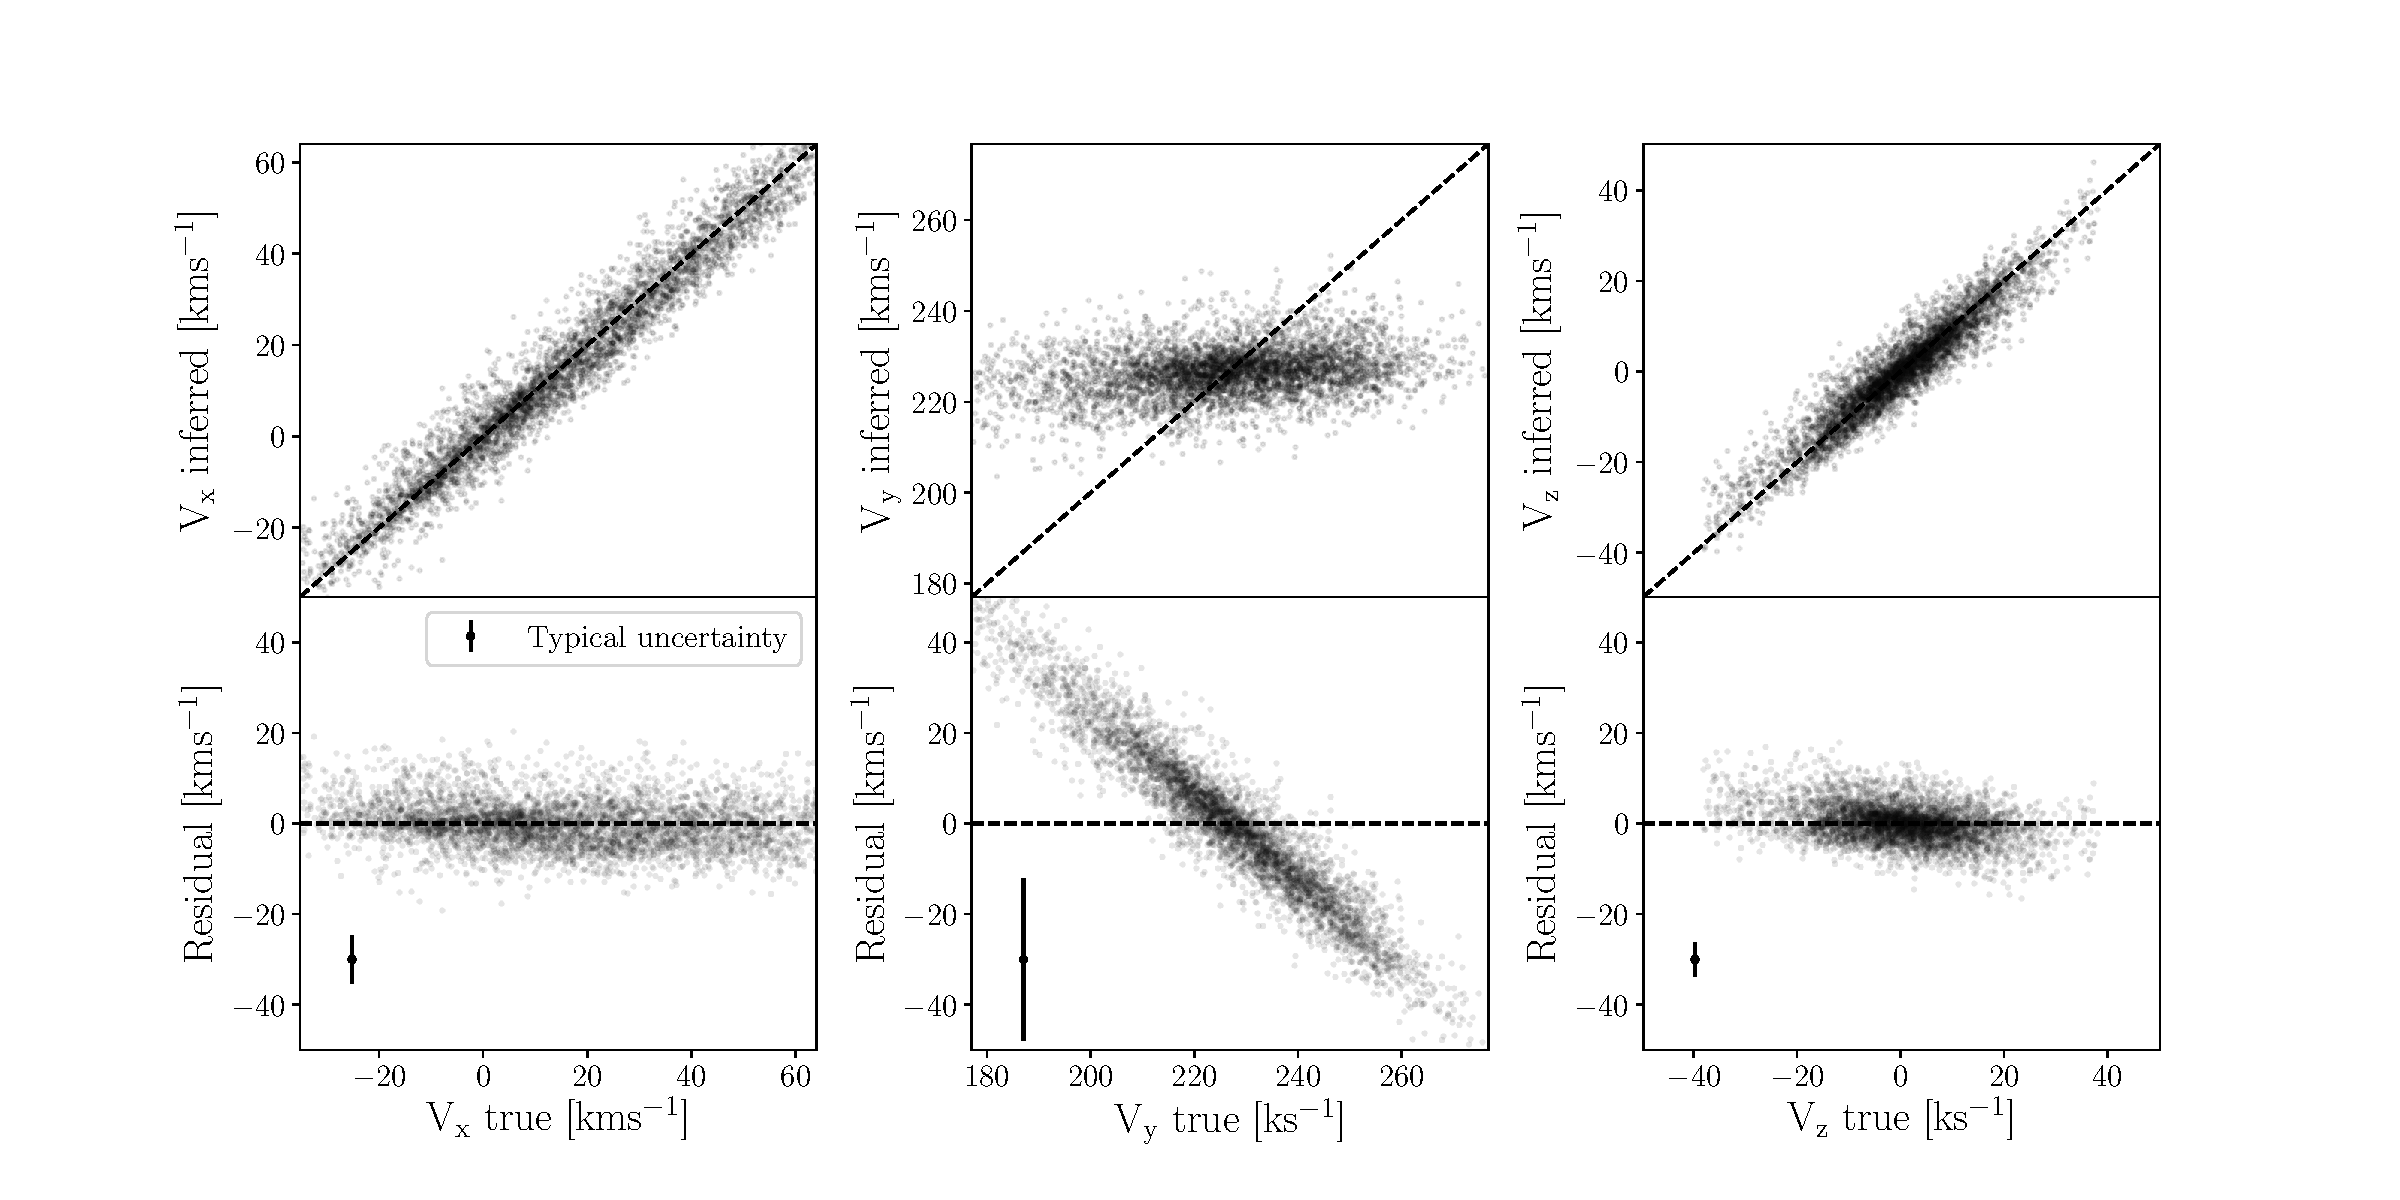
\includegraphics[width=1\textwidth]{residuals}
\label{fig:residuals}
\end{figure}
The \kepler\ field is oriented almost along the \y\-axis of the Galactocentric
coordinate system.
As a result, \x\ and \z-direction velocities of \kepler\ stars are extremely
well-constrained with proper motion alone, but \vy\ is almost completely
unconstrained without an RV.
Figure \ref{fig:v_comparison} shows that \vx\ and \vz\ velocities inferred
without RV measurements are extremely similar to those calculated with RVs.
